\documentclass{article}
\usepackage[utf8]{inputenc}
\usepackage[english]{babel}

\usepackage{amsfonts}
\usepackage{amsthm}
\usepackage{tikz}
\usetikzlibrary{shapes.arrows,chains}

\theoremstyle{definition}
\newtheorem{definition}{Definition}[section]
\newtheorem{example}{Example}[section]

\begin{document}

\section{Two problems}
Firstly we shall look at two problems which belong to the complexity class NP.

\subsection{Traveling Sales Person}
Consider a finite set $N$ of cities; $\{1, 2 \dots n\}$. The distance, or cost,
of traveling between cities $i$ and $j$ is given by $D(i,j)$ where $D$
is a symmetric matrix.

$$\forall i, j\quad D(i,J) \in \mathbb{N}\quad D(i,j) = D(j,i)$$

The problem is to find a path, or permutation, of
cities where each city appears exactly once in the path and the total
cost is minimised.

The brute force solution is to consider all paths, doing this would require
considering $!n$ paths.

\subsection{Boolean Formula Satisfiability}
A boolean formula consists of the logical binary operators $(\land, \lor, \neg)$
and a finite set of variables $X$ where each variable can be either true or false.
The problem consists of deciding if there exists a set of values for the variables $X$
which results in the boolean formula being true.

$$(x_1 \land x_2) \land \neg x_3$$

$$(x_1 \land x_2) \land \neg x_1$$

A brute force solution would be to consider all $2^{|X|}$ possible assignments.

\section{Turing Machines}
What do Turing machines do? Why are we looking at them?

Conceptually a turing machine is a \textit{tape} which is infinite in both directions,
the input is writen on this tape with the rest of the tape being blank. We have a head
which can read and write to the tape. The machine moves across the tape acording to
a transition function until it reaches a terminal state which produces a yes or no result.

\begin{center}
	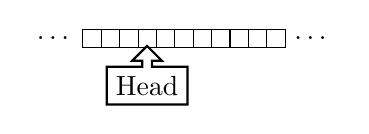
\begin{tikzpicture}[
	  start chain=1 going right,start chain=2 going below,node distance=-0.15mm
	]
		\node [on chain=1] at (-1.5,-.4) {\ldots};
		\foreach \x in {1,2,...,11} {\x, \node [draw,on chain=1] {}; }
		\node [
			name=k,
			arrow box,
			on chain=2,
			arrow box arrows={north:.25cm},
			draw=black,thick
			] at (-0.335,-1) {Head};
		\node [name=r,on chain=1] {\ldots};
	\end{tikzpicture}
\end{center}


\begin{definition}
	Formally a Turing machine consists of
	\begin{itemize}
		\item A \textit{tape alphabet} $\Gamma$ $\{a_1, a_2 \dots a_n, \beta\}$,
			where $a_i$ is a symbol, and $\beta$ is the blank or empty symbol.
		\item An \textit{input alphabet} $\Sigma$
			where $\Sigma \subset \Gamma \setminus \{\beta\}$.
		\item A set of states $Q$ $\{q_0, q_1 \dots q_m, q_y, q_n\}$ where $q_0$ is the
			initial state, $q_y$ is the terminal yes state, and $q_n$ is the terminal no state.
			$Q\prime = Q \setminus \{q_y,q_n\}$, i.e. the non-terminal states.
		\item A transition function $\delta$,
			where $\delta\ :\ (Q\prime \times \Gamma) \rightarrow
			(Q \times \Sigma \times \{L,S,R\})$.
			What this means is we look at a pair of a non-terminal state
			and a symbol from the alphabet;
			given this we enter a new state $q \in Q$,
			we write to the tape a symbol $a \in \Gamma$,
			and we stay or move the head left or right $(\{L,S,R\})$.
	\end{itemize}
\end{definition}

\subsection{An example}
\begin{example}
	In this example we will present a turing machine to decide if a number is even.
	\begin{itemize}
		\item Input: a number $x \in \mathbb{Z}$ in unary form; i.e. $\{1 = X, 2 = XX\dots\}$,
			thus $\Sigma = \{X\}$.
		\item Output: yes iff $x$ is even, otherwise no. I.e. the turing machine will finish
			in state $q_y$ iff $x$ is even.
		\item Transition function $\delta$ is described as a matrix below with the states
			$Q\prime = \{q_0,q_1\}$ and $\Sigma = \{X,\beta\}$,
			output is $(Q \times \Sigma \times \{L,S,R\})$.
		\begin{center}
			\begin{tabular}{ c c c }
					 & $q_0$           & $q_1$           \\
				X    & ($q_1,\beta,R$) & ($q_0,\beta,R$) \\
			 $\beta$ & ($q_y,\beta,S$) & ($q_n,\beta,S$) \\
			\end{tabular}
		\end{center}
	\end{itemize}
\end{example}

Now the important thing about the above example is how many times the transition function is applied

Bit on worst case vs average vs best case

\subsection{Recognising Palindromes}

\end{document}
